\documentclass[12pt,a4paper]{article}

\usepackage{geometry}
\usepackage[T1]{fontenc}
\usepackage{mathpazo} % Palatino font
\usepackage{microtype} % Better typography
\usepackage{textcomp} % For proper dash support
\usepackage{amsfonts}
\usepackage{amsmath}
\usepackage{graphicx}
\usepackage{float}
\usepackage{hyperref}
\hypersetup{
    colorlinks=true,
    linkcolor=black,
    filecolor=magenta,
    urlcolor=blue,
    citecolor=black,
}

% Additional packages for figures
\usepackage{tikz}
\usetikzlibrary{shapes,arrows,positioning,fit,backgrounds,calc,decorations.pathreplacing} % For Conceptual Model
\usepackage{pgfgantt} % For Timeline
% float package is already loaded above
\usepackage{xcolor} % Usually included by tikz or pgfgantt, but good to ensure

% Typography settings
\linespread{1.05} % Slightly increased line spacing
\setlength{\parindent}{1.5em}
\setlength{\parskip}{0.5em}
\setlength{\textwidth}{6.5in}
\setlength{\textheight}{9in}
\setlength{\oddsidemargin}{0in}
\setlength{\evensidemargin}{0in}
\setlength{\topmargin}{0in}
\setlength{\headheight}{15pt}
\setlength{\headsep}{40pt}
\setlength{\footskip}{30pt}

% Additional typography packages
\usepackage{ragged2e}
\usepackage{booktabs}
\usepackage[inline]{enumitem}
\usepackage{multicol}
\usepackage{multirow}
\usepackage{appendix}
\usepackage{tabularx}
\usepackage{threeparttable}
\usepackage{pdflscape}
\usepackage{array}
\usepackage{setspace}
\usepackage{fancyhdr}
\usepackage[sorting=none,backend=biber]{biblatex}

\addbibresource{main.bib}

\pagestyle{fancy}
\fancyhf{}
\fancyhead[L]{Methods of Research}
\fancyhead[R]{Spring 2025}
\fancyfoot[C]{\thepage}

%%%%%%%%%%%%%%%%%%%%%%%%%%%%%%%%%%%%%%%%%%%%%%%%%%
% ENTER GROUP AND PROJECT INFORMATION
%%%%%%%%%%%%%%%%%%%%%%%%%%%%%%%%%%%%%%%%%%%%%%%%%%

\newcommand{\grouptitle}{Group 1 - Research Proposal}
\newcommand{\studentone}{Student Name 1}
\newcommand{\studenttwo}{Student Name 2}
\newcommand{\studentthree}{Student Name 3}
\newcommand{\projecttitle}{Agent Protocol Primitives for \\Digital Twins of Human Operators in Distributed Energy Resource Systems}
\newcommand{\submissiondate}{June 7, 2025}
\newcommand{\emdash}{\textemdash}

%%%%%%%%%%%%%%%%%%%%%%%%%%%%%%%%%%%%%%%%%%%%%%%%%%

\begin{document}

% Title Page
\begin{titlepage}
\begin{center}
{\Huge Research Proposal} \\
\vspace{5mm}
{\Large Methods of Research} \\

\vspace{10mm}

{\huge\textbf{\projecttitle}} \\

\vspace{15mm}

\hrule
\vspace{3mm}
\begin{tabular}{ll}
\textbf{Group Members:} & {\studentone} \\
& {\studenttwo} \\
& {\studentthree} \\
\\
\textbf{Submission Date:} & {\submissiondate} \\
\textbf{Word Count:} & 2,588 words (excluding abstract) \\
\end{tabular}
\vspace{3mm}
\hrule

\vspace{15mm}

\textbf{Abstract} \\
\vspace{2mm}
\begin{minipage}{0.8\textwidth}
\textbf{Abstract:} This research investigates how emerging agent protocol primitives\emdash{}specifically the Model Context Protocol (MCP), Agent Communication Protocol (ACP), and Agent-to-Agent Protocol (A2A)\emdash{}can be adapted and integrated with Digital Twin principles to create Human DER Worker Digital Twins (HDTs). The study addresses operational challenges in Distributed Energy Resource (DER) management, including communication gaps, coordination difficulties, and the need to simulate human operational behaviors in increasingly automated environments. Through a systematic literature review and compositional framework development, this research proposes an unexplored approach to modeling human operational behaviors within protocol-enabled digital twins, with potential applications for preserving and scaling operational patterns across distributed energy systems. The expected contributions include a validated framework for Human DER Worker Digital Twins, insights into protocol composition for energy system operator coordination, and processes for implementing human-centric digital twins in energy system operations.
\end{minipage}

\end{center}
\end{titlepage}

\newpage

\clearpage

\section{Introduction and Background}
\label{sec:introduction}

The transformation of global energy systems toward decentralized architectures presents unprecedented operational challenges that fundamentally alter how maintenance activities must be coordinated and executed \cite{10.1109/ACCESS.2024.3387400}. The proliferation of Distributed Energy Resources (DERs)\emdash{}including rooftop solar installations, battery storage systems, and wind microgeneration\emdash{}has created a complex multi-stakeholder ecosystem where traditional centralized maintenance approaches prove inadequate \cite{10.1016/j.rser.2020.110607}.

\subsection{Problem Context and Significance}

The DER ecosystem involves diverse stakeholders with varying technical capabilities, business objectives, and operational constraints. Individual homeowners with rooftop solar installations operate under different knowledge bases and decision-making frameworks than commercial facility managers, utility operators, or industrial microgrid controllers \cite{10.1016/j.seta.2022.102837}. This heterogeneity creates significant challenges in preserving, transferring, and scaling human operational behaviors across the distributed energy landscape.

Current approaches to DER coordination rely heavily on centralized Distributed Energy Resource Management Systems (DERMS), which struggle to capture and utilize the nuanced human operational behaviors required for effective system operations \cite{10.1049/iet-gtd.2019.1022}. Increasing automation of energy systems requires bridging the gap between human operational patterns and automated decision-making processes. Human experts possess tacit knowledge about equipment behavior, environmental factors, stakeholder coordination patterns, and operational trade-offs, but also exhibit operational uncertainties and inconsistencies that cannot be easily codified within traditional control systems \cite{10.1080/095281300146308}.

The significance of this challenge extends beyond operational efficiency to encompass workforce and sustainability considerations. The aging workforce in the energy sector faces retirement without adequate knowledge transfer mechanisms, risking the loss of decades of operational experience and behavioral patterns \cite{10.1109/ETFA61755.2024.10711109}. Effective preservation and scaling of human operational behaviors directly impacts grid stability, renewable energy integration, and the democratization of energy systems \cite{10.3390/en14154579}. Moreover, the COVID-19 pandemic has highlighted the importance of resilient energy infrastructure that can maintain operations despite disruptions to traditional mentoring and knowledge transfer workflows.

The challenge is particularly acute in DER operations where human operational behaviors encompass complex coordination patterns—understanding how to balance homeowner preferences with grid stability requirements, how to prioritize competing operational demands under uncertainty, and how to adapt to local environmental and regulatory constraints \cite{10.1109/ACCESS.2024.3387400}. Traditional one-on-one mentoring approaches fail to scale across distributed operations \cite{10.1007/s44163-022-00020-w}, and formal documentation systems cannot capture the tacit knowledge and operational uncertainties of operators in dynamic, multi-stakeholder environments \cite{10.1016/j.apergo.2018.07.016}.

\subsection{Literature Review Synthesis}

A preliminary literature review across four domains\emdash{}human factors in energy systems, industry-academia collaboration, AI automation applications, and safety training methodologies\emdash{}reveals consistent patterns pointing toward the need for more sophisticated human-technology integration in DER management.

\textbf{Human Factors and Communication Gaps:} Research in nuclear power plant operations demonstrates that human expertise remains critical for managing complex, safety-critical systems \cite{10.1108/13552510610654510}. Studies of control room operators highlight the importance of tacit knowledge, situational awareness, and adaptive decision-making that cannot be fully automated \cite{10.1049/OAP-CIRED.2017.1107}. In DER contexts, similar patterns emerge where human operators must navigate between technical system requirements and real-world operational constraints.

\textbf{Digital Twin Technology in Energy Systems:} The application of Digital Twin technology in energy systems has shown promising results for system optimization and operational coordination \cite{10.1016/j.esr.2024.101334}. However, existing implementations focus primarily on physical asset modeling rather than capturing human operational patterns and expertise. Recent reviews identify the need for "Human Digital Twins" that can model operator behavior and decision-making processes \cite{10.1109/ETFA61755.2024.10711109}.

\textbf{Agent Protocol Primitives:} Emerging agent protocol primitives, particularly MCP, ACP, and A2A, offer new possibilities for distributed coordination and knowledge sharing \cite{10.5220/0001894702000205}. These protocols enable more sophisticated multi-agent interactions than traditional approaches, supporting complex negotiation, resource sharing, and collaborative problem-solving patterns essential for DER coordination.

\subsection{Research Gap Identification}

The literature synthesis reveals three critical gaps that this research addresses:

\textbf{Theoretical Gap:} Current Digital Twin frameworks lack comprehensive models for representing human operational behaviors within protocol-enabled environments. While Digital Twins excel at modeling physical systems, they fail to capture the tacit knowledge, adaptive reasoning, operational uncertainties, and contextual decision-making patterns that human experts bring to DER operations.

\textbf{Methodological Gap:} Existing agent protocol primitives have not been systematically evaluated for their effectiveness in modeling human operational behaviors including both expertise and uncertainty patterns. The lack of standardized approaches for integrating human behavioral patterns within agent-based systems limits the development of more effective human-AI collaboration models.

\textbf{Practical Gap:} The DER industry lacks validated frameworks for creating Human DER Worker Digital Twins that can model human operational behaviors across distributed operations while maintaining the adaptability, contextual awareness, and inherent uncertainties that characterize human expert performance, with potential for future scaling applications.

These gaps represent a significant barrier to realizing the full potential of DER systems for sustainable energy transition. Without effective mechanisms for modeling and potentially preserving human operational behaviors including their uncertainties, the increasing automation of energy systems risks losing critical operational patterns while failing to achieve the coordination necessary for large-scale renewable energy integration.

\section{Research Objectives and Questions}
\label{sec:objectives}

\subsection{Research Objectives}

\textbf{Overarching Research Objective:} This research aims to develop and validate a framework for creating Human DER Worker Digital Twins (HDTs) using agent protocol primitives to effectively model human operational behaviors in Distributed Energy Resource operations.

\textbf{Objective 1:} Identify and structure the essential components of Human DER Worker operational behaviors\emdash{}including tools, knowledge resources, communication patterns, and uncertainty management\emdash{}that can be effectively modeled and represented within an HDT framework using agent protocol primitives.

\textbf{Objective 2:} Design and evaluate protocol-enabled HDT architectures that can model various Human DER Worker behaviors within specific DER Application Contexts such as operational knowledge management and stakeholder interaction.

\textbf{Objective 3:} Develop a comprehensive evaluation framework for assessing HDT effectiveness across technical efficacy, representation fidelity, and human factors dimensions.

\subsection{Primary Research Questions}

\textbf{Overarching Research Question:} How can agent protocol primitives (specifically MCP, ACP, and A2A) be adapted and integrated with Digital Twin principles to create Human DER Worker Digital Twins that effectively model human operational behaviors?

\textbf{Question 1:} What are the essential components of a Human DER Worker's operational behaviors that can be effectively identified, structured, and modeled within an HDT framework using agent protocol primitives?

\textbf{Question 2:} How can different agent protocol architectures be effectively mapped and implemented to model various Human DER Worker behaviors within specific DER Application Contexts such as operational knowledge management and stakeholder interaction?

\textbf{Question 3:} What multi-faceted evaluation framework is required to assess the impact of HDT integration on DER operations, and how does performance feedback contribute to refining HDT representations?

\section{Scope and Limitations}
\label{sec:scope}

This research is bounded by the following scope and limitations:

\textbf{Protocol Focus:} The analysis and conceptual design will be strictly limited to the application and adaptation of MCP, ACP, and A2A protocols. Other agent protocols or general communication standards will not be explored in detail.

\textbf{Use Case Specificity:} The research focuses solely on modeling human operational behaviors for DERs through digital twins. Applications in other DER functions such as energy trading or grid stability services are outside the scope.

\textbf{Framework Development:} The research will develop a structured framework for HDT creation and evaluation rather than building fully operational software systems.

\textbf{Implementation Constraints:} This proposal-stage research will not include full-scale system implementation or field deployment testing.

\textbf{Validation Scope:} Validation will be conducted through literature-based analysis and conceptual framework evaluation rather than empirical field studies.

\textbf{Stakeholder Coverage:} The research focuses primarily on technical operators and maintenance personnel, with limited attention to policy makers or regulators. Whether to include other stakeholders will be determined by the research findings.

\section{Theoretical Framework}
\label{sec:framework}

\subsection{Core Conceptual Model}

The theoretical framework is structured around concepts operating within two primary domains: Reality (Human-Centric) and Digital Twin (Protocol-Enabled). This framework directly addresses theoretical gaps identified in current digital twin research \cite{10.1186/s10033-024-00998-7} \cite{10.1016/j.ifacol.2022.09.675}.

\begin{figure}[h!]
    \centering
    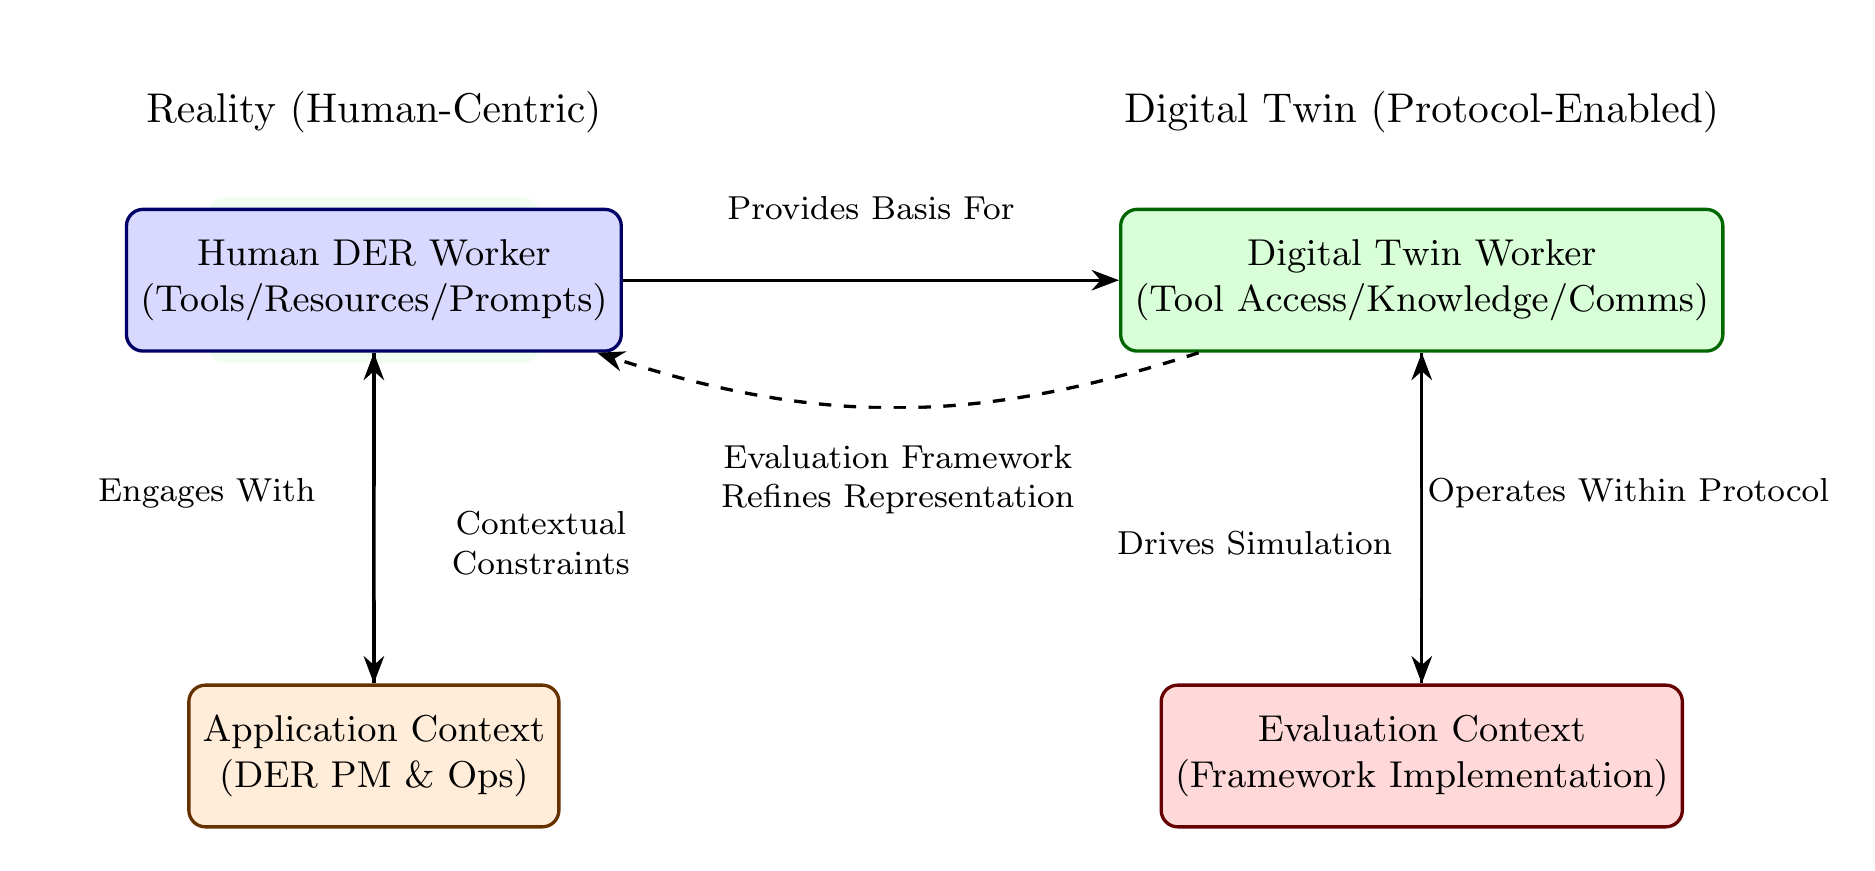
\includegraphics[width=\linewidth]{conceptual-model-diagram-1.png}
    \caption{Conceptual Model of Human DER Worker Digital Twins}
    \label{fig:conceptual-model}
\end{figure}

\textbf{Human DER Worker (Tools/Resources/Prompts):} The fundamental human element encompassing operational behaviors, tools (SCADA interfaces, diagnostic equipment), knowledge resources (technical manuals, historical data, regulatory frameworks), and communication patterns (SOPs, reporting formats, escalation pathways). Current literature reveals significant gaps in representing cognitive processes within industrial environments \cite{10.1007/s44163-022-00020-w} \cite{10.1016/j.apergo.2018.07.016}, highlighting inadequate formalization for the operational uncertainties that characterize human expert performance in complex operational contexts.

\textbf{Application Context (DER Operational Knowledge Management):} The operational environment where DER systems require behavioral pattern preservation and transfer across distributed locations and stakeholders, characterized by distributed system complexity and real-world operational constraints.

\textbf{Digital Twin Worker (Tool Access/Knowledge/Communications):} An agent-based software system that models and replicates human DER worker operational behaviors through structured protocols, featuring tool access layers, AI-driven natural language uncertainty, and standardized communication protocols built using MCP, A2A, and domain-specific protocols. Current Digital Twin frameworks focus predominantly on physical asset modeling, with limited theoretical development for integrating human behavioral modeling with technical system representations \cite{10.1016/j.esr.2024.101334} \cite{10.1007/s10207-023-00784-x}.

\textbf{Evaluation Context (Framework Implementation):} The systematic assessment framework for validating HDT effectiveness through fidelity metrics, operational efficiency measures, human factors validation, and safety outcomes assessment. No comprehensive theoretical framework currently exists for evaluating the effectiveness of human digital twins in operational contexts \cite{10.1109/etfa61755.2024.10711109} \cite{10.1016/j.ifacol.2022.09.675}.

\subsection{Framework Integration and Theoretical Contributions}

The four core concepts operate within a structured interaction model where Human-Centric Reality provides foundational operational behaviors, Protocol-Enabled Digital Twins model and augment human behavioral patterns, bidirectional relationships facilitate learning and refinement, and evaluation frameworks validate effectiveness and drive iterative improvement. This framework addresses the identified gaps in agent protocol composition for human behavioral modeling and dynamic human-AI collaboration models, providing theoretical foundations for protocol architecture design that consider human operational behavior modeling requirements and bidirectional learning mechanisms between human experts and their digital twin representations.

\section{Research Methodology}
\label{sec:methodology}

\subsection{Methodological Approach}

This research employs a multi-phase methodology combining systematic literature review, compositional framework development, and rapid prototyping approaches. This methodology addresses the nascent validation frameworks for human-centric digital twins \cite{10.1109/etfa61755.2024.10711109}, limited integration of multi-disciplinary methodologies \cite{10.1016/j.ifacol.2022.09.675}, and insufficient real-world operational context integration \cite{10.1007/s10207-023-00784-x}.

\textbf{Phase 1: Systematic Literature Review (6-8 weeks):} Systematic analysis of protocol composition patterns and integration approaches, focusing on agent protocol primitives in DER contexts and human behavioral modeling techniques. This phase addresses the identified limitation of a lack of multi-disciplinary integration across human factors engineering, digital twin technology, and energy systems management domains.

\textbf{Phase 2: Compositional Framework Development (8-10 weeks):} Systematic analysis of how MCP, ACP, and A2A protocols can be integrated and composed for HDT implementation, developing an architectural framework that map protocol capabilities to different HDT functional layers for modeling human operational behaviors. This phase provides systematic methodology for evaluating multi-protocol agent architectures in human-centric applications.

\textbf{Phase 3: Proof of Concept Development (4-6 weeks):} Rapid prototyping of framework components to demonstrate behavioral modeling feasibility and validate conceptual models through structured scenarios. This stage tests the practical demonstration and validation of the framework on current protocol primitives against operational scenarios.

\subsection{Addressing Methodological Limitations}

The proposed methodology addresses the limitations identified in Digital Twins research approaches \cite{10.1186/s10033-024-00998-7} \cite{10.1016/j.ifacol.2022.09.675}. The multi-phase approach explores various aspects of the new protocol primitives by combining multiple research methodologies. The compositional framework development phase establishes validation frameworks for HDT effectiveness using protocol primitives, addressing the problem of prior methodologies focusing solely on physical system fidelity without considering human operational behavior modeling.

\subsection{Alternative Methodologies Considered}

\noindent \textbf{Design Science Research:} While offering comprehensive framework development capabilities, this approach was deemed inadequately suited to address the time constraints and resource limitations identified in methodological limitations analysis, ranking lower in feasibility assessment.

\noindent \textbf{Action Research:} Considered for its emphasis on stakeholder inclusion but excluded due to lacking systematic framework development capabilities needed for theoretical contribution, and inadequate integration of multi-disciplinary requirements.

\noindent \textbf{Grounded Theory:} Evaluated for theory development potential but deemed inappropriate given the existing theoretical foundation and the need for multi-disciplinary integration requirements identified in the limitations analysis.

\subsection{Quality Assurance}

Methodology validation addresses identified limitations through multi-disciplinary validation across research domains, systematic documentation addressing reproducibility limitations, operational context connection maintaining relevance to real-world implementation requirements, and structured feedback mechanisms. Regular milestone reviews, systematic documentation of design decisions, cross-validation of findings against established literature, and structured feedback from domain experts ensure comprehensive quality assurance that overcomes the methodological constraints identified in current HDT-related research.

\section{Ethics and Sustainability}
\label{sec:ethics}

\subsection{Ethical Considerations}

\noindent \textbf{Data Privacy and Human Expertise:} The modeling of human expertise raises important questions about intellectual property rights and the potential commodification of tacit knowledge. The research will address consent frameworks for expertise capture and establish guidelines for respectful representation of human capabilities.

\noindent \textbf{Human-AI Collaboration Ethics:} The development of HDTs must avoid creating systems that replace human workers rather than augmenting their capabilities. Ethical guidelines will ensure that HDT implementations preserve human agency and decision-making authority in critical operational contexts.

\noindent \textbf{Algorithmic Transparency:} Agent-based systems must maintain transparency in their decision-making processes to ensure human operators can understand and validate automated recommendations.

\subsection{Sustainability Integration}

\noindent \textbf{Environmental Dimensions:} This research directly supports UN Sustainable Development Goal 7 (Affordable and Clean Energy) by improving the operational efficiency of renewable energy systems and enabling more effective integration of distributed clean energy resources.

\noindent \textbf{Social Sustainability:} The preservation and scaling of human operational behaviors supports workforce development and knowledge transfer, contributing to SDG 4 (Quality Education) and SDG 8 (Decent Work and Economic Growth).

\noindent \textbf{Economic Sustainability:} Enhanced DER coordination reduces operational costs and improves system reliability, supporting the economic viability of energy transitions.

\section{Risk Assessment and Implementation Plan}
\label{sec:risks}

\subsection{Risk Management}

\noindent \textbf{High Priority Risks:}
\begin{itemize}
\item \textbf{Scope Creep (Probability: Medium, Impact: High):} Mitigation through clearly defined protocol focus and regular scope reviews.
\item \textbf{Limited Access to Proprietary Protocols (Probability: Medium, Impact: Medium):} Mitigation through emphasis on publicly available protocol specifications and academic literature.
\item \textbf{Complexity of Human Expertise Modeling (Probability: High, Impact: Medium):} Mitigation through incremental framework development and focus on well-documented expertise domains.
\end{itemize}

\noindent \textbf{Medium Priority Risks:}
\begin{itemize}
\item \textbf{Literature Quality Variability:} Addressed through systematic quality assessment criteria and multiple validation sources.
\item \textbf{Rapid Technology Evolution:} Managed through focus on fundamental protocol principles rather than implementation-specific details.
\end{itemize}

\subsection{Implementation Timeline}

\textbf{Weeks 1-8:} Systematic literature review and gap analysis completion.
\textbf{Weeks 9-16:} Compositional framework development and protocol analysis.
\textbf{Weeks 17-20:} Proof of concept development and validation.

\textbf{Key Milestones:}
\begin{itemize}
\item Week 4: Literature review methodology validation
\item Week 8: Comprehensive gap analysis completion
\item Week 12: Initial framework architecture design
\item Week 16: Compositional protocol analysis completion
\item Week 20: Final framework validation and documentation
\end{itemize}

\begin{figure}[h!]
    \centering
    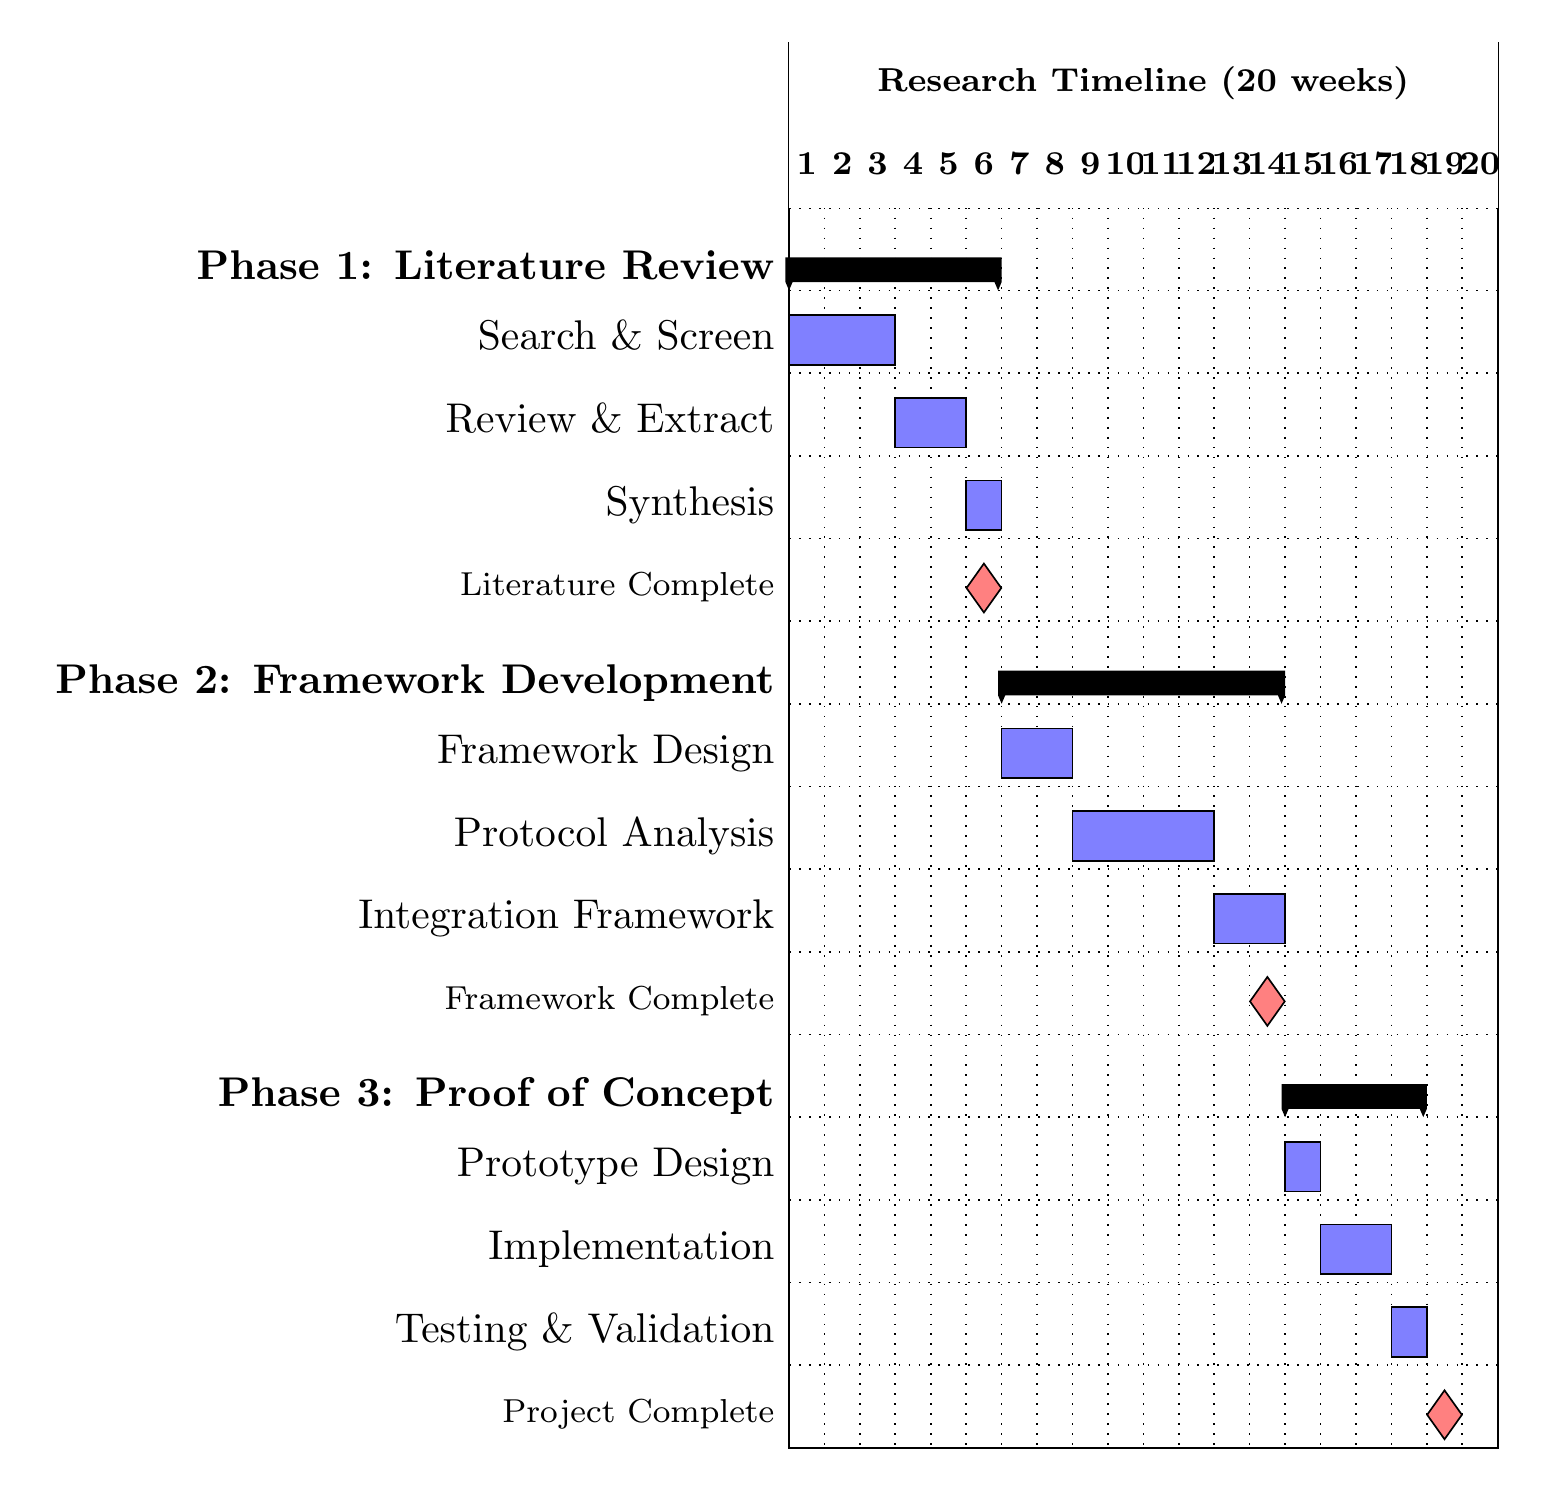
\includegraphics[width=.8\linewidth]{timeline-gantt-simple-1.png}
    \caption{Research Implementation Timeline}
    \label{fig:timeline}
\end{figure}

\section{Expected Results and Contributions}
\label{sec:results}

\subsection{Anticipated Outcomes}

\noindent \textbf{Theoretical Contributions:} A validated framework for Human DER Worker Digital Twins that bridges human operational behavior modeling and agent protocol primitives, providing novel insights into protocol composition for multi-agent coordination in energy systems.

\noindent \textbf{Methodological Contributions:} Systematic methodology for evaluating agent protocols in human behavioral modeling contexts, including validation criteria and implementation guidelines for HDT development.

\noindent \textbf{Practical Contributions:} Detailed reference for DER industry practitioners seeking to implement human-centric digital twins, including protocol selection, implementation processes, and evaluation frameworks.

\subsection{Impact and Significance}

The research is expected to advance both the theoretical understanding and practical implementation of human-centered digital twins in energy systems. The framework will provide a foundation for practical value in simulations for DER operators seeking to scale operational behaviors across distributed operations, while offering a look at future research potentials in language-based AI implementation in the energy sector.

The integration of agent protocol primitives with Digital Twin technology represents a novel or unexplored approach to addressing the challenge of preserving and scaling human operational behaviors in energy systems. This research contributes to the broader goal of sustainable energy transition by developing frameworks that could improve the operational efficiency and reliability of distributed renewable energy systems through better preservation of human operational patterns.

\clearpage

% Bibliography
\printbibliography

\end{document}